\documentclass[a4paper,11pt,uplatex]{jsbook}

%\usepackage{fancyhdr}
\setlength{\footskip}{16pt}
\usepackage{amsmath}
\usepackage[dvipdfmx]{graphicx}
\usepackage[dvipdfmx]{color}
%\usepackage{pagecolor}[white]
\usepackage{amsmath,amssymb}
%\usepackage[top=3cm, bottom=3cm, left=3cm, right=3cm]{geometry}
\usepackage{braket}
\usepackage{bm}
\numberwithin{equation}{section}
\usepackage{mathrsfs}
\usepackage{siunitx}
\usepackage{physics}
\usepackage[dvipdfmx]{graphicx}
\usepackage[compat=1.1.0]{tikz-feynhand}
\usepackage{caption}
\usepackage{subcaption}
%\usepackage{cleveref}
\usepackage{float}
\usepackage{multicol}
\setlength{\columnsep}{15mm}
%\usepackage[style=phys,articletitle=false,biblabel=brackets,chaptertitle=false,pageranges=false]{biblatex}
%\usepackage[style=phys]{biblatex}
\usepackage[dvipdfmx]{hyperref}
\usepackage{url}
\usepackage{pxjahyper}
\usepackage{bookmark}
%\usepackage[backref]{hyperref}
\setcounter{tocdepth}{3}
\setlength{\parindent}{2em}
\def\vector#1{\mbox{\boldmath $#1$}}
\def\slash#1{\not\!#1}
\def\slashb#1{\not\!\!#1}
\def\delsla{\not\!\partial}
%\usepackage[dvipdfmx]{xcolor}


\hypersetup{
 setpagesize=false,
 bookmarksnumbered=true,%
 bookmarksopen=true,%
 colorlinks=true,%
 linkcolor=black,
 citecolor=red,
 urlcolor=black,
}
%backreferenceのカスタマイズ. "Back to p.3"のように表示する.
%\renewcommand*{\backref}[1]{(p.#1へ戻る)}
%\newcommand{\backtoc}{\hyperlink{toc}{[目次へ]}}
\newcommand{\backtoc}{\texorpdfstring{\protect\hyperlink{toc}{\hspace{5pt} \scriptsize [目次へ]}}{}}
\newcommand{\mychapter}[1]{\chapter[#1]{#1\backtoc}}
\newcommand{\mysection}[1]{\section[#1]{#1\backtoc}}
\newcommand{\mysubsection}[1]{\subsection[#1]{#1\backtoc}}
% 数式
%\usepackage{amsmath,amsfonts}
%\usepackage{bm}
%\usepackage{physics}
% 画像
%\usepackage[dvipdfmx]{graphicx}
%\usepackage[dvipdfmx,colorlinks=true,linkcolor=blue]{hyperref}
%\usepackage{pxjahyper}
\begin{document}


\chapter{アンジュレータ放射光干渉法の原理}
アンジュレータ放射光干渉法の概要を以下の図に示す。
%図を入れる
初めに\ref{sec:undulator}章でアンジュレータ放射光の発生原理と放射される放射光の性質を述べる。
続いて\ref{sec:tandem}節以降で2台のアンジュレータを用いることによる干渉の原理を示す。軸上($\theta =0$)放射の場合と、一般の$\theta$におけるエネルギー決定公式を導く。
続いて\ref{sec:optics}章で放射光観測のための光学系による光学処理の原理を示す。
最後にこれらの原理をまとめた完全な物理モデルによる関数系の概要を示す。
\section{アンジュレータ放射光}
高エネルギーの荷電粒子が磁場中を通過するなどして加速度運動をすると、シンクロトロン放射光と呼ばれる電磁波が発生する。
特に素粒子実験や加速器設計の立場からは、シンクロトロン放射によるエネルギー損失は無視できない問題であった。
一方、電磁石の磁場を用いることで人為的に放射光を発生させ、利用する技術が開発されてきた。
シンクロトロン放射は一般に指向性が高く極めて強い放射光を得ることができるため、物性科学や生物科学、医学などの広い分野で分光法やイメージング法に利用されている。

さらに、偏極電磁石による円軌道からの放射だけでなく、周期的な磁場を用いることでより高輝度で単色性の放射光が得られることが知られている。このような周期的磁場の発生装置を
ウィグラーやアンジュレータと呼び、特に電子ビームラインに挿入する形で用いられることから挿入光源と総称される。
アンジュレータ放射光干渉法はこのアンジュレータを利用した電子ビームエネルギー測定法である。
次節ではまず、放射光の発生原理について述べる。

\subsection{アンジュレータ放射光発生の原理}\label{sec:undulator}
この節ではアンジュレータの原理を示す。

\subsubsection{放射光の一般原理}\label{sec:general radiation}
リエナール・ヴィーヘルト・ポテンシャルから出発して、放射強度の角分布についての一般的な性質を説明する。電子から観測点へ向かうベクトルを$\bm{R}$、これに平行な単位ベクトルを$\bm{n} = \bm{R}/R$、電子の電荷$e$、電子の相対論的速度$\bm{\beta} = \bm{v}/c$、
放射が発生した時刻(遅延時刻)$t'$、放射の観測時刻$t$として
\begin{eqnarray}
  \bm{A}(t) &=& \frac{\mu_0 c}{4\pi}\frac{e\bm{\beta(t')}}{(1-\bm{n}(t')\cdot\bm{\beta}(t'))\bm{R}(t')}\label{retarded potential}\\
  \varphi(t) &=& \frac{1}{4\pi \epsilon_0}\frac{e}{(1-\bm{n}(t')\cdot\bm{\beta}(t'))\bm{R}(t')}\label{retarded potential phi}\\
  t &=& t' + \frac{R(t')}{c}
\end{eqnarray}
放射される電磁場は、電磁ポテンシャルの定義より得ることができる。
\begin{eqnarray}
  \bm{E} &=& -\bm{\nabla} \varphi - \frac{1}{c}\frac{\partial \bm{A}}{\partial t}\\
  \bm{B} &=& \bm{\nabla} \times \bm{A}
\end{eqnarray}
したがって、電磁場は
\begin{eqnarray}
  \bm{E} &=& \frac{e}{4\pi \epsilon_0}\left( \frac{(1-\beta^2)(\bm{n}(t')-\bm{\beta}(t'))}{R(t')^2(1-\bm{n}(t')\cdot\bm{\beta}(t'))^3}+
  \frac{\bm{n}(t')\times \left\{ (\bm{n}(t')-\bm{\beta}(t'))\times \bm{\dot{\beta}}(t')\right\}}{cR(t')(1-\bm{n}(t')\cdot\bm{\beta}(t'))^3} \right)\\
  \bm{B} &=& \frac{\bm{n}\times\bm{E}}{c}
\end{eqnarray}
と与えられる。$1/R(t')^2$の項は遠方で無視できるとして簡単にすると、
\begin{eqnarray}\label{eq:e field}
  \bm{E} &=& \frac{e}{4\pi \epsilon_0}\frac{\bm{n}(t')\times \left\{ (\bm{n}(t')-\bm{\beta}(t'))\times \bm{\dot{\beta}}(t')\right\}}{cR(t')(1-\bm{n}(t')\cdot\bm{\beta}(t'))^3}\\
  \bm{B} &=& \frac{\bm{n}\times\bm{E}}{c}
\end{eqnarray}
放射強度はポインティングベクトル$\bm{S} =\bm{E}\times \bm{B}/\mu_0 = |\bm{E}|^2\bm{n}/c\mu_0$を用いて、$\text{d}P(t) = (\bm{S}\cdot\bm{n})R^2\text{d}\Omega$と表される。
ただし、このままでは左辺が$t$の関数として与えられているのに対し、右辺は$t'$の関数であり扱いづらい。ここでは$t'$に統一して、
\begin{eqnarray} \label{eq:power}
  \frac{\text{d}P(t')}{\text{d}\Omega} = \frac{\text{d}P(t)}{\text{d}\Omega}\frac{\text{d}t}{\text{d}t'} = \frac{e^2}{16\pi^2 \epsilon_0 c}\frac{\left|\bm{n}\times \left\{ (\bm{n}-\bm{\beta})\times \bm{\dot{\beta}}\right\}\right|^2}{(1-\bm{n}\cdot\bm{\beta})^5}
\end{eqnarray}

\begin{figure}[htbp]
  \centering
  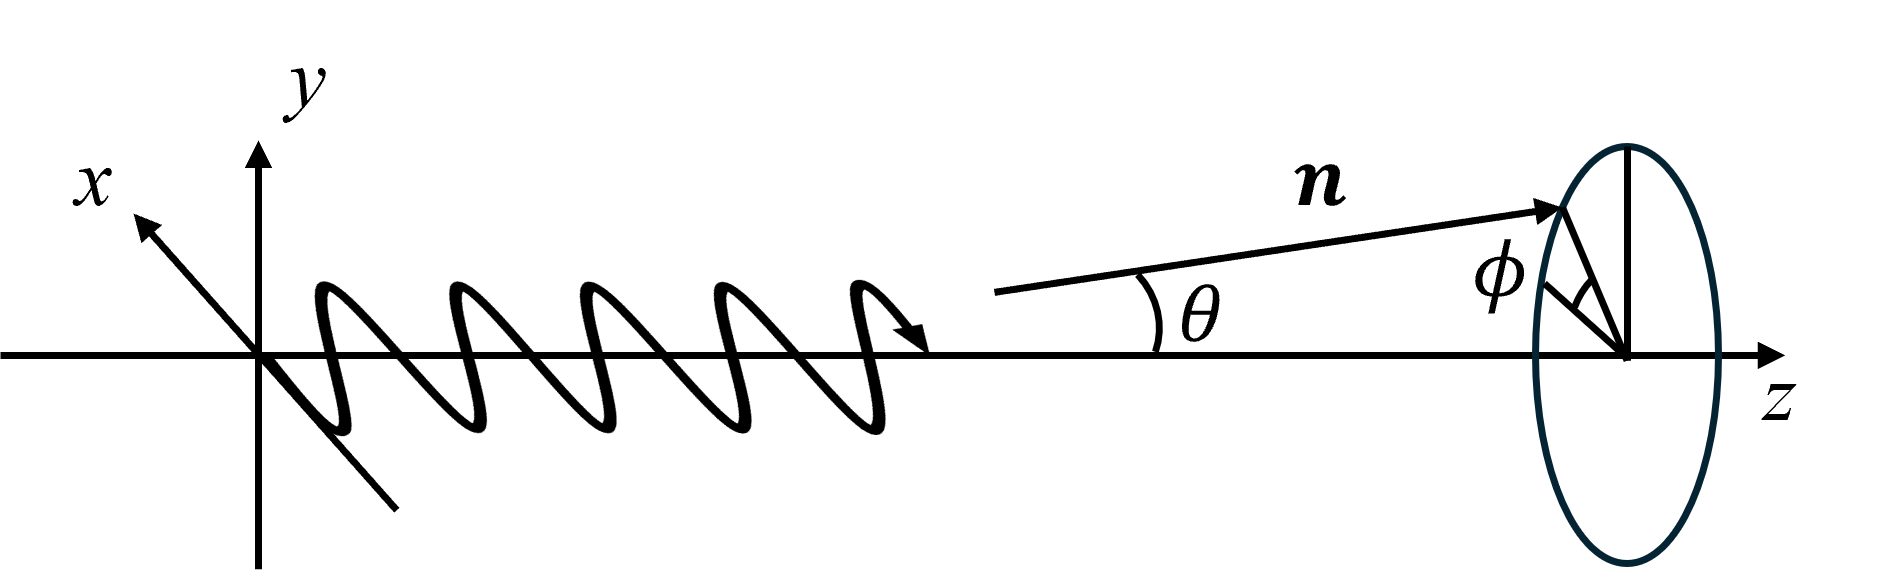
\includegraphics[width=10cm]{image/2-cordinate.png}
  \caption{座標系}
\end{figure}
%アンジュレータであることを一言入れる。
今はアンジュレータの磁場による偏向運動を考えたいため、$\bm{\beta} \perp \bm{\dot{\beta}}$として議論を進める。
電子の運動方向を$z$軸にとり$\bm{\beta} = (0,0,\beta)$とする。また、磁場が$y$軸に向いているとすれば、$\bm{\dot{\beta}} = (\dot{\beta},0,0)$とおける。3次元極座標表示で、$\bm{n} = (\sin\theta\cos\phi,\sin\theta\sin\phi,\cos\theta)$とすると、
\begin{eqnarray}\label{eq:power2}
  \frac{\text{d}P(t')}{\text{d}\Omega} = \frac{e^2\dot{\beta}^2}{16\pi^2 \epsilon_0 c}\frac{(\cos\theta - \beta)^2 + (1-\beta^2)\sin^2\theta\sin^2\phi}{(1-\beta \cos\theta)^5}
\end{eqnarray}
$\beta \simeq 1$ の時に式(\ref{eq:power2})の分母が$\theta \ll 1$で0に近づくことにより、放射強度は電子の進行方向に鋭く集中することがわかる。$\theta \ll 1$のもとで$(1-\beta\cos\theta)^{-1}$が最大値の1/2になる角度を$\theta_{SR}$とすると、
\begin{eqnarray}
  \theta_{SR} = \sqrt{2\left(\frac{1}{\beta} -1\right)} \sim \frac{1}{\gamma}
\end{eqnarray}
となり、この角度より狭い円錐の中に放射強度の大部分が集中することがわかる。
%電子のローレンツ因子の逆数よりも狭い角度に集中する。
%ここで、$\gamma$は電子のローレンツ因子である。

\subsubsection{アンジュレータの周期的磁場による放射}\label{sec:undulator radiation}
アンジュレータによって発生させられた周期的な磁場$B = B_0 \sin(2\pi z/\lambda_u)$中を電子が運動すると、同じ周期長$\lambda_u$を持つ正弦波状の軌道を描き、いわゆる蛇行(undulation)運動をする。
この磁場中の電子の運動方程式を解くと、電子の速度および位置を
\begin{eqnarray}\label{eq:undulator motion}
  \beta_x &=& \frac{K\beta}{\gamma}\cos(\omega_0 t')\\
  \beta_z &=& \beta\left[1 - \frac{K^2}{4\gamma^2} -\frac{K^2\cos (2\omega_0 t')}{4\gamma^2} \right]\\
  r_x &=& \frac{K\lambda_U}{2\pi \gamma}\sin(\omega t')\\
  r_z &=& \left(1-\frac{K^2}{4\gamma^2}\beta c t'\right) - \frac{K^2\lambda_U \sin(2\omega_0 t')}{16\pi \gamma^2}
\end{eqnarray}
と得ることができる。ここで
\begin{eqnarray}
  \omega_0 = 2\pi c\beta \frac{1-K^2/4\gamma^2}{\lambda_U}
\end{eqnarray}
であり、$K$は偏向定数と呼ばれ、電子軌道の最大偏角$\Psi$と
\begin{eqnarray}
  K = \gamma \Psi = \frac{eB_0\lambda_u}{2\pi m c^2} = 93.4 \frac{B_0}{[\text{T}]}\frac{\lambda_u}{[\text{m}]}
\end{eqnarray}
のように関係づけられる。表式からわかるように、アンジュレータの周期と磁場によって偏向定数が決まる。

アンジュレータ放射は偏向定数によって特徴づけられる。電子軌道は最大偏角$\Psi = K/\gamma$のサイン型であり、\ref{sec:general radiation}節で述べたように、放射強度の広がりは$1/\gamma$程度となることから、
$K \sim 1$の場合には電子からの放射はほとんどすべて観測者に到達する。この時の電場はほぼサイン型になり、フーリエ変換して得られるスペクトルは単色性を持つ。このような放射をアンジュレータ放射と呼ぶ。
一方、$K \gg 1$の場合には、電子がサイン型軌道の頂点を通過するときにのみ放射が観測されるため、大きくゆがんだパルス状になる。フーリエ変換によって得られるスペクトルは高調波が卓越する。このような放射をウィグラー放射と呼ぶ。
このように偏向定数によって放射特性を変化させることができ、実用上は磁場強度を変化させることで求められる特性の放射を取り出すことができる。

また放射スペクトル、すなわち放射強度の周波数($\omega$)分布を求めたい。そのためには式\ref{eq:e field}に\ref{eq:undulator motion}を代入し、電場の時間変化を得たうえでフーリエ変換を行えばよい。
電場のフーリエ変換は観測点における周波数成分を求めることに対応するため
\begin{eqnarray}
  \bm{F}(\omega) = \int_{-\infty}^{\infty} \bm{E}(t')\exp(-i\omega t)dt
\end{eqnarray}
とすれば、全放射強度の角密度は
\begin{eqnarray}
  \frac{\text{d}W}{\text{d}\Omega} = \int_{-\infty}^{\infty} \frac{\text{d}P(t)}{\text{d}\Omega}dt = \frac{1}{2c\mu_0\pi}\int_{0}^{\infty} \left|R\bm{E}\right|^2 dt 
  = \frac{1}{c\mu_0}\int_{-\infty}^{\infty} \bm{F}(\omega)\bm{F}(\omega)^*d\omega
\end{eqnarray}
と変形できる。一方で、単位周波数当たりの全放射強度は
\begin{eqnarray}
  \frac{\text{d}W}{\text{d}\Omega} = \int_{0}^{\infty}\frac{\text{d}^2I}{\text{d}\omega \text{d}\Omega}\text{d}\omega
\end{eqnarray}
したがって
\begin{eqnarray}
  \frac{\text{d}^2I}{\text{d}\omega \text{d}\Omega} = \frac{1}{2c\mu_0\pi}\bm{F}(\omega)\bm{F}(\omega)^*
\end{eqnarray}
ただし遅延時刻$t'$で評価された式も観測時刻$t$でフーリエ変換されていることに注意する。$\bm{n} =(\sin\theta\cos\phi,\sin\theta\sin\phi,\cos\theta)$を再び用いると、$\bm{n}\perp\bm{E}$であるから、
$\bm{n}$に垂直な2成分だけなので、特に$x-z$平面と平行な成分$E_{\parallel}$およびこれに垂直な成分$E_{\perp}$に分解することができる。フーリエ変換した結果は次のように表せる。
\begin{eqnarray}
  E_\parallel &=& g\xi\left\{2S_0\gamma \theta \cos\phi - K (S_1 + S_{-1})\right\}\\
  E_\perp &=& g\xi\left\{2S_0\gamma \theta \sin \phi\right\}
\end{eqnarray}
この式で、$N$をアンジュレータの周期数として、
\begin{eqnarray}
  g &=& -i \frac{e\gamma}{cR} \frac{\sin \left( N\pi (\omega/\omega_1 -1) \right)}{\omega/\omega_1 -1}\exp\left[-ik\omega_1 R/c \right]\\
  \omega_1 &=& \frac{2\gamma^2\omega_0}{1+K^2/2 + (\gamma\theta)^2}\\
  \xi &=& \frac{1}{1 + (\gamma\theta)^2 + K^2/2} \\
  S_q &=& \sum_{p = -\infty}^{\infty} J_{1+2p+q}(2\xi K\gamma\theta\cos\phi)J_p(K^2/4)
\end{eqnarray}
であり、$J_p$は$p$次のベッセル関数である。このようにして、アンジュレータ放射光のスペクトルを求めることができる。
\begin{eqnarray}\label{eq:spectrum}
  \begin{split}
   \frac{\text{d}^2I}{\text{d}\omega \text{d}\Omega} &= \frac{e^2\gamma^2\xi^2}{\pi^2 c}\frac{\sin^2 \{N\pi(\omega/\omega_1 -1)\}}{(\omega/\omega_1 -1)^2}\\
   &~~~~~~~~~~~~~~\times\left[ \{2S_0\gamma\theta\cos\phi - K(S_1 + S_{-1})\}^2 + \{2S_0\gamma \theta \sin \phi\}^2 \right]
  \end{split}
\end{eqnarray}

最後に、電場の時間変化について簡単な計算を行う。$\theta = 0$で観測することを考える
アンジュレータの入口に到達する時刻を$t' = t'_1 $、アンジュレータの出口から出る時刻を$t' = t'_2$とする。アンジュレータの長さを$L$とすれば、
$t'_2 - t'_1 \simeq L / v$と書ける。さらにアンジュレータの出口から観測点までの距離を$R$とすれば、電場の時間変化の始まりと終わりを検知する時刻は、
$t_1 = t'_1 + (R + L)/c$、$t_2 = t'_2 + R/c$と書ける。したがって観測者が検知するパルス幅$\Delta t$は、$v/c \simeq 1- 1/2\gamma^2$を考慮して
\begin{eqnarray}
  \Delta t = t_2 - t_1 = \frac{L}{v}  - \frac{L}{c} \simeq \frac{L}{2c\gamma^2}
\end{eqnarray}
同様の計算は、アンジュレータの1周期について行うことも可能であり、電場変化の周期は$L\rightarrow \lambda_U$の変換によって求められる。
電場変化の周期はアンジュレータの磁場変化の周期に対応することから、アンジュレータ放射の時間構造は磁場と同じ回数振動するパルス状の波形になる。
アンジュレータ内の蛇行運動によって$z$軸方向の平均の相対論的速度は式\ref{eq:undulator motion}より$<\beta_z> =\beta (1-K^2/4\gamma^2)$であることがわかり、結果として観測される放射の周期は
\begin{eqnarray}
  T &=& \frac{\lambda_U}{v(1-K^2/4\gamma^2)} \\
  &=& \frac{\lambda_U}{2c\gamma^2}(1 + K^2/2)
\end{eqnarray}
したがってアンジュレータ放射の波長は
\begin{eqnarray}
  \lambda_L = \frac{\lambda_U}{2\gamma^2}(1+K^2/2)
\end{eqnarray}
にピークを持つようなスペクトルを持つことがわかる。

\subsection{アンジュレータ放射光 - タンデムアンジュレータ}\label{sec:tandem}
アンジュレータを電子ビームに沿って2つ連結した構成は放射光科学において広く使われている。
これらのアンジュレータ間にシケイン電磁石を配置することで遅延を調整することが可能になる。
アンジュレータの種類や構成によって位相や偏光状態の異なる様々な形状の放射光を得ることができる。

本研究では、タンデムアンジュレータを用いる。アンジュレータ自体を移動させることでアンジュレータ間の物理的距離を変化させる点が特徴的な構成である。

\subsection{干渉の原理}\label{sec:interference}
\ref{sec:undulator radiation}節の議論を応用すると、タンデム型アンジュレータから放射される放射光はダブルパルス型の波形となることがわかる。
そのままでは2つのパルスは干渉することができないため、遅延を発生させる必要がある。この役割を担っているのが回折格子である。
回折格子のそれぞれの溝から散乱された光は格子間隔に比例して遅延された光の干渉となる。
そのためダブルパルスの二つのパルスは格子による遅延を受けて干渉できることになる。
\begin{figure}[b]
  \centering
  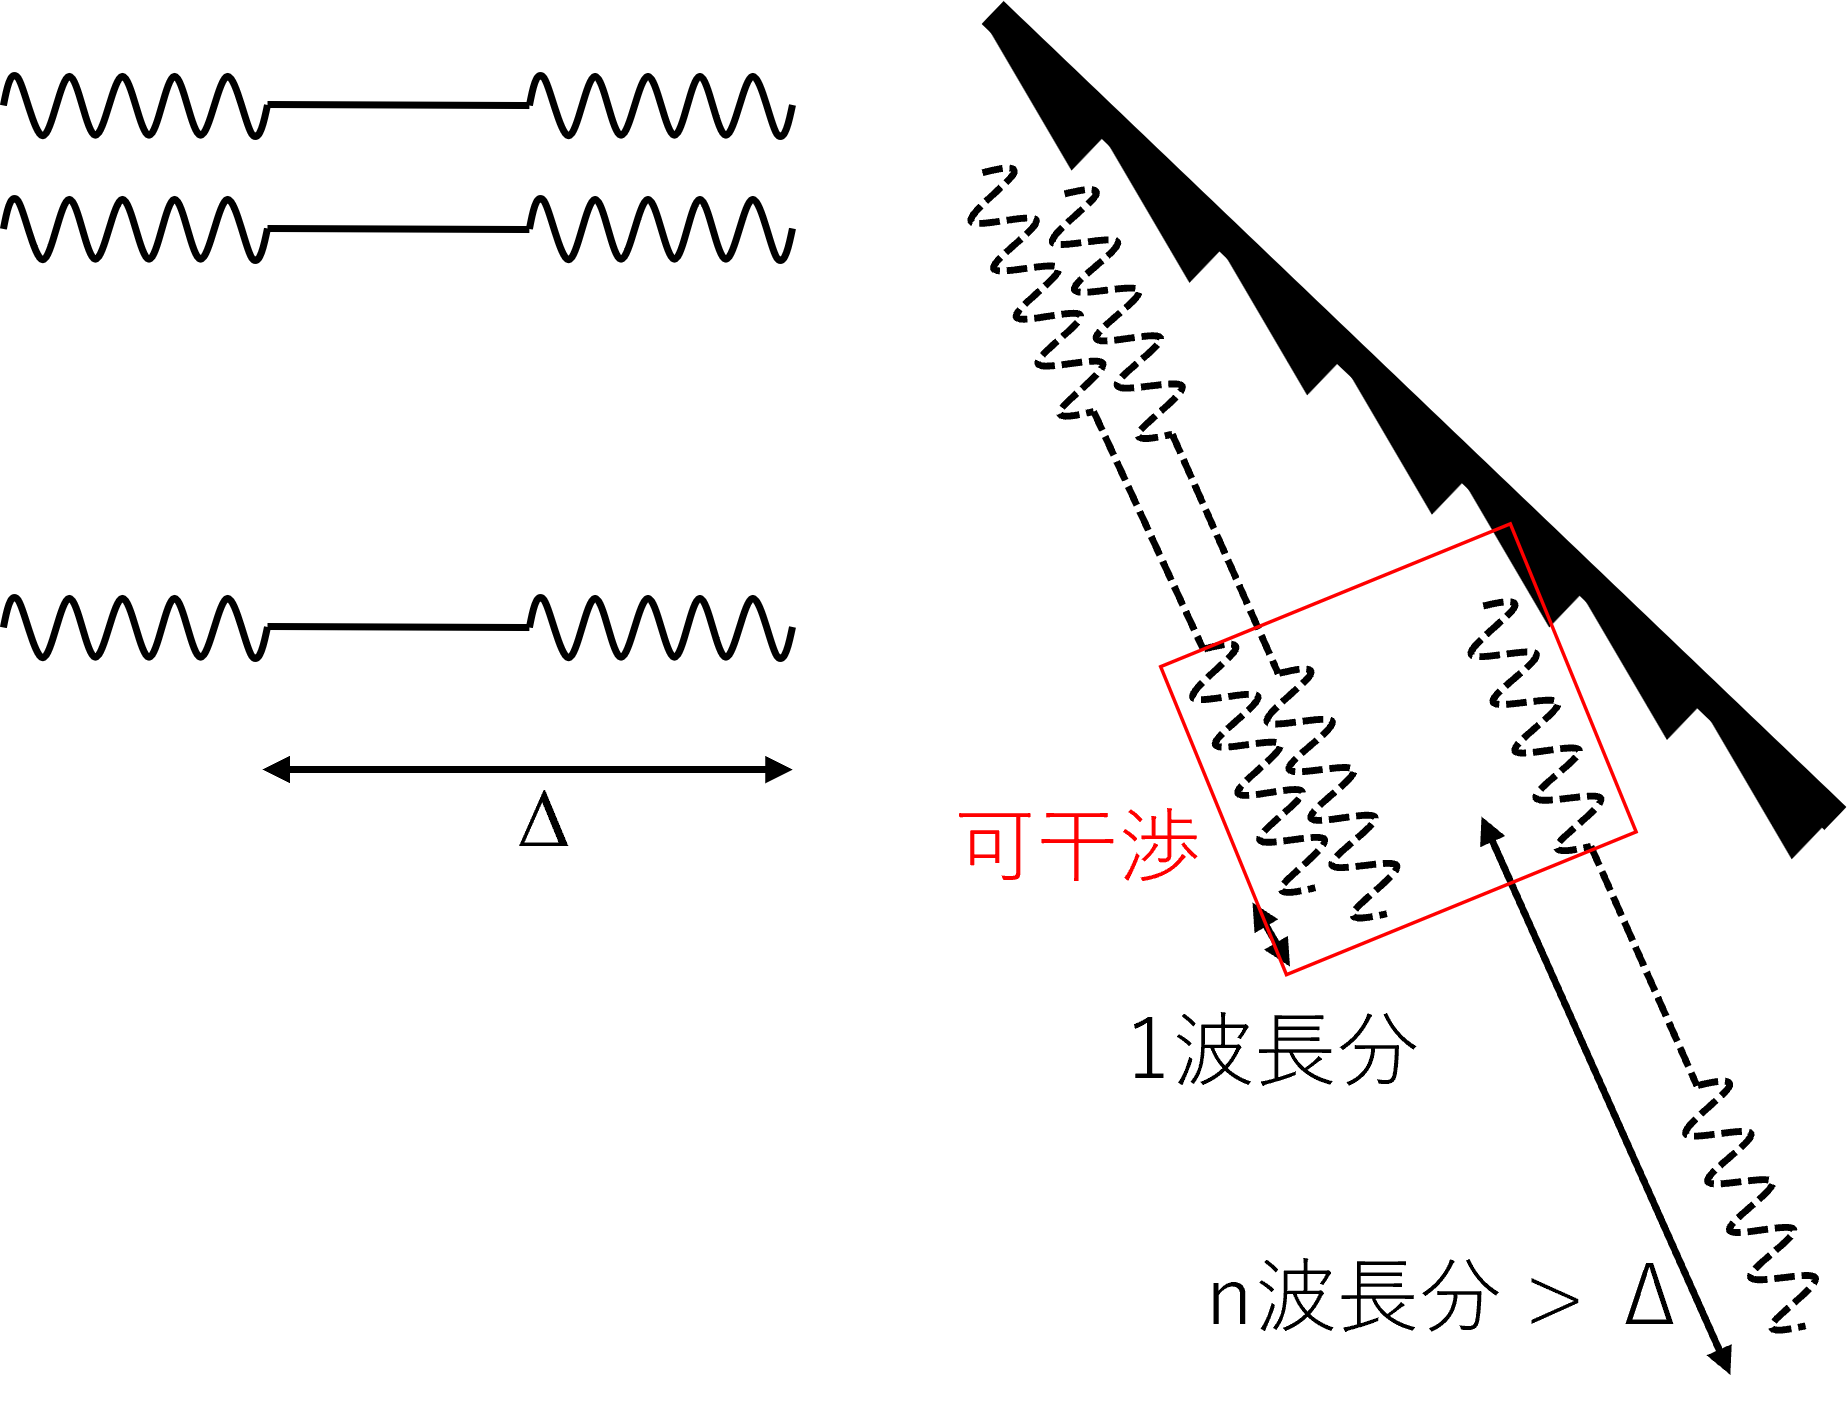
\includegraphics[width=10cm]{image/2-doublepulse.png}
  \caption[干渉の原理]{ダブルパルス間の間隔以上の遅延が回折格子の溝同士で起きれば、パルス同士の干渉作用を観測することができる。}
  \label{fig:doublepulse}
\end{figure}

\subsection{電子ビームエネルギーと干渉光周期の関係式}
ダブルパルスの間隔は以下のような近似で理解することができる。
\begin{figure}
  \centering
  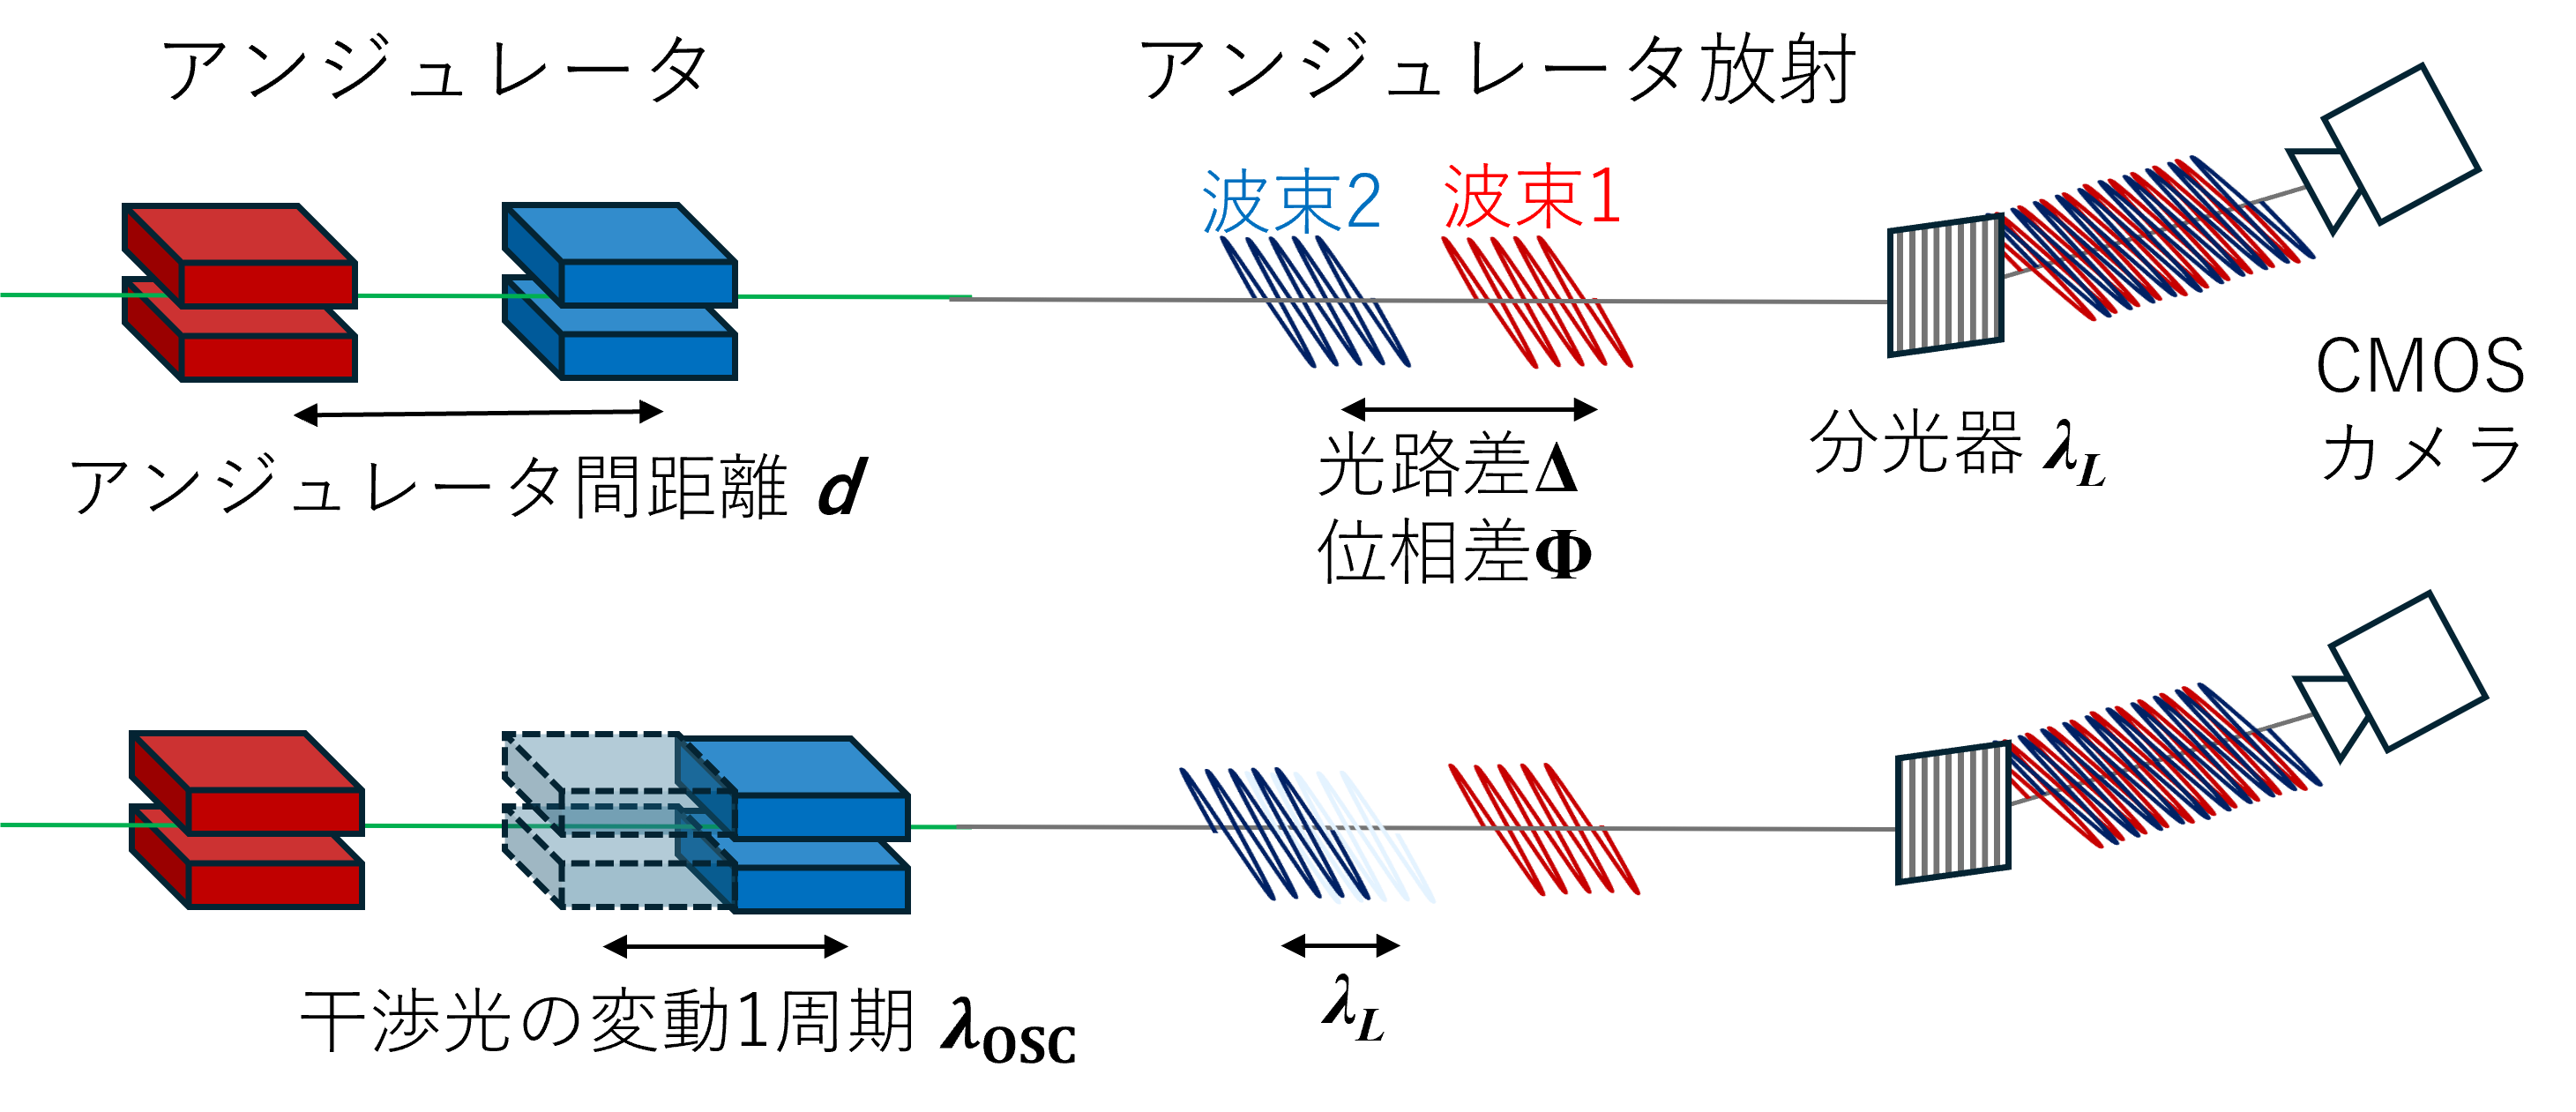
\includegraphics[width=10cm]{image/2-lambdaosc.png}
  \caption{アンジュレータ放射光干渉法の概要}
\end{figure}
上流のアンジュレータで発生する放射光は電子ビームよりも早く、電子が下流側のアンジュレータに到達した時にはアンジュレータ間の距離に比例した光路差が生じる。
\begin{eqnarray}
  \Delta = \frac{1}{2\gamma^2}d \label{path shift}
\end{eqnarray}
この時間差は放射光の2つのパルスの位相差となる。
\begin{eqnarray}
  \Phi = 2\pi \frac{\Delta}{\lambda_L}
\end{eqnarray}
位相差に対応して干渉光は強めあい、干渉光強度は
\begin{eqnarray}
  |\tilde{E} \left( 1+ e^{i\Phi}\right)|^2 
&= |\tilde{E}|^2 \left( 1 + \cos(\Phi) \right)\\
&= |\tilde{E}|^2 \left( 1 + \cos(\frac{2\pi}{2\gamma^2\lambda_L}d) \right) 
  \label{oscillation}
\end{eqnarray}
これより、dを変化させると干渉光の位相差が変化し強度が周期的に変動することがわかる。
式(\ref{oscillation})から、アンジュレータ間距離を$2\gamma^2\lambda_L$だけ動かした時に1周する。
この周期を$\lambda_{osc}$とおけば$\gamma$および電子ビームエネルギーが
\begin{eqnarray}
  \gamma = \sqrt{\frac{\lambda_{\text{osc}}}{2\lambda_L}}\\
  \text{E}_\text{beam} =m_e c^2  \sqrt{\frac{\lambda_{\text{osc}}}{2\lambda_L}} \label{zero order energy formula}
\end{eqnarray}\label{eq:energy_prim}
すなわち、干渉光の波長$\lambda_L$と、アンジュレータ間距離を変動させた時の干渉光の変動の周期$\lambda_{\text{osc}}$
を精密に測定することで電子ビームエネルギーが精密に測定できる。

\subsection{補正 - 放射角度と干渉光周期の関係式}
式(\ref*{path shift})は放射光角度が電子ビームと同じとき($\theta$ =0)の光路差である。
電子ビームの軸と放射光の放射角(近似的に放射光の観測角)を$\theta$とおくと、
アンジュレータ間の距離$d$と$\theta$で光路差が$d(1-\cos{\theta})$と表される。
これと電子ビームの遅延による光路差の両方を考慮した光路差は、
\begin{eqnarray}
  \Delta &= d\frac{1}{2\gamma^2} + d(1 - \cos{\theta}) \\
        &\sim d(\frac{1}{2\gamma^2} + \frac{\theta^2}{2})\\
\end{eqnarray}
と表せる。したがって放射光の観測角($\simeq$ 放射角)の補正を入れることで干渉光の周期は
\begin{eqnarray}
  \lambda_{\text{osc}} = \frac{\lambda_L}{\frac{1}{2\gamma^2} + \frac{\theta^2}{2}}
\end{eqnarray}
となる。

より現実に即した計算として、放射光の振幅と位相を式に従って計算し、スリット直前での干渉光をy座標の関数として表したのが図??である。
下流アンジュレータの位置に対して周期的な変動が見られる。
またy座標は放射角に対応しており、周期的変動の周期、位相が放射角に依存していることがわかる。


\section{光学系}\label{sec:optics}
放射光は光学系を通してカメラで光学的に撮影する。光学系の役割は分光とパルス波形の平面化にある。
式(\ref{zero order energy formula})が示すとおり、
電子ビームエネルギーは波長に依存するため$10^{-4}$のエネルギー絶対値較正精度を得るために波長決定精度は少なくとも$10^{-4}$程度必要となる。
またタンデムアンジュレータから放射される放射光は\ref{sec:undulator radiation}節で示したようにダブルパルス型の波形を持ちこのままでは2つのパルスは干渉を起こさない。
そのため平面波化(フーリエ変換)が必要となる。
図\ref{optics_schematic}に光学系の概要を示す。
\begin{figure}[b]
  \centering
  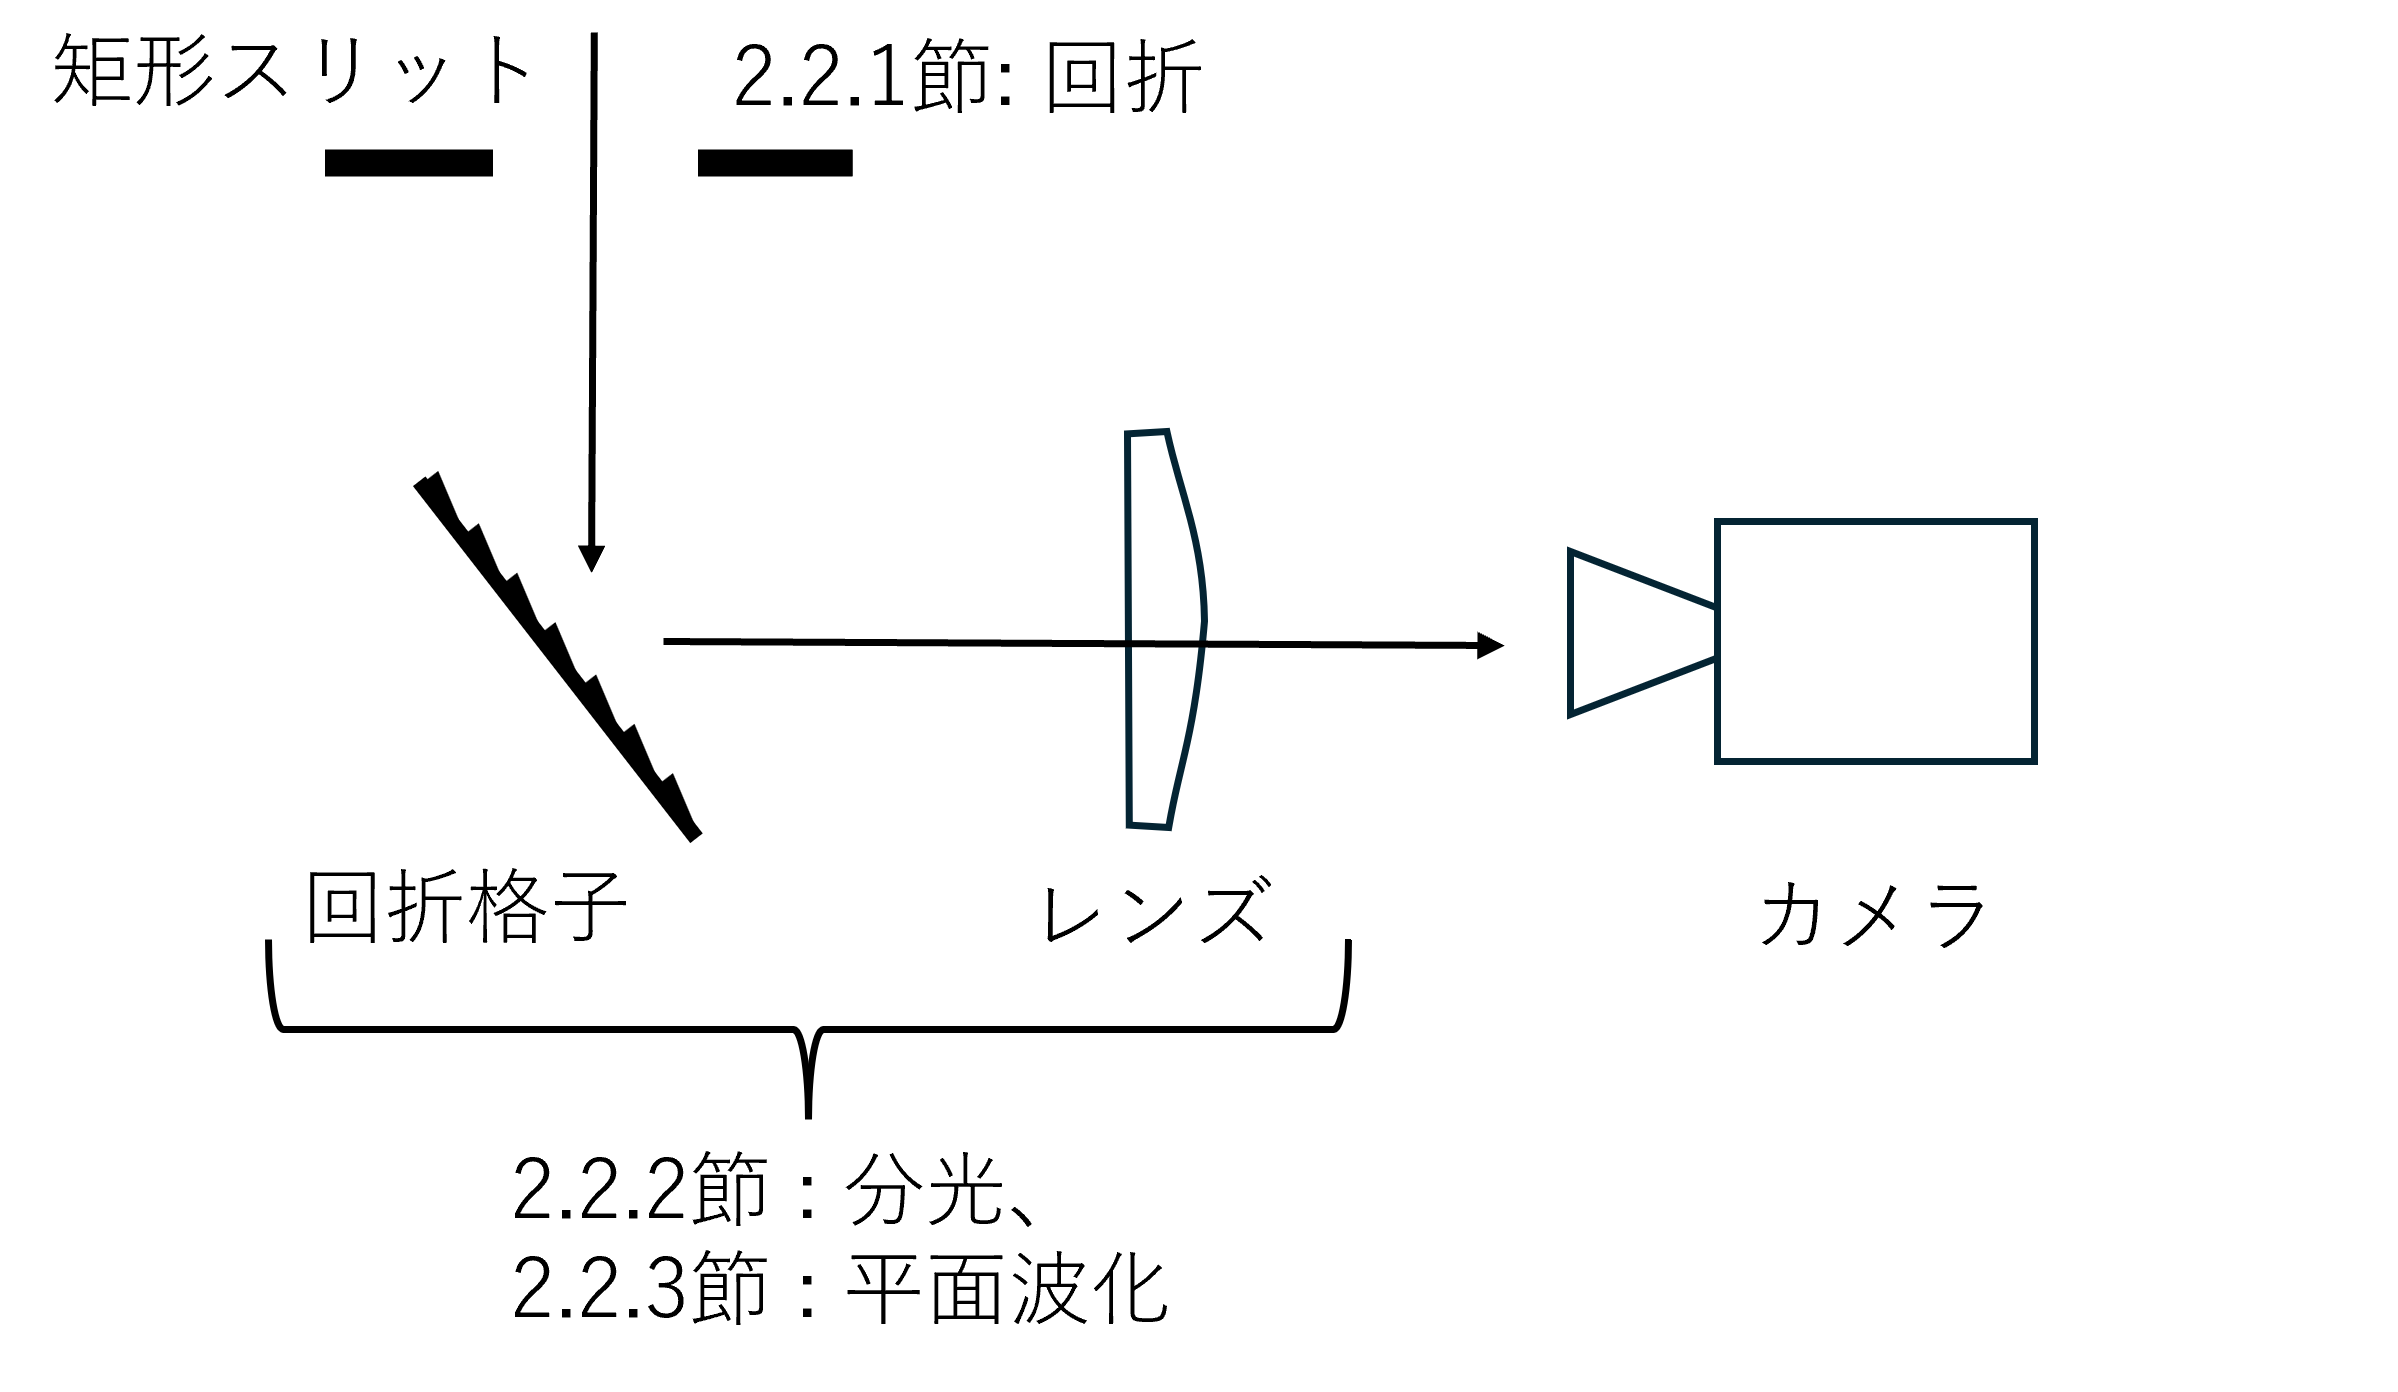
\includegraphics[width=10cm]{image/2-opticsshematic.png}
  \caption{光学系の概要}
  \label{optics_schematic}
\end{figure}
矩形スリットで整形した光波は伝搬に伴って回折を生じる(\ref{sec:rayleigh}章)。後段には回折格子およびレンズがあり、
光波は分光と平面波化(\ref{sec:grating},\ref{sec:grating2}章)を受けカメラに到達する。

\subsection{レイリー・ゾンマーフェルト回折積分}\label{sec:rayleigh}
光波の伝搬はマクスウェル方程式に従う。
ある平面の波面から別の平面での波面を計算するには、レイリーゾンマーフェルト回折積分が知られている。
今回のセットアップにおいては近軸近似を用いることで、スクリーンでの回折パターンを式(??)によって計算できる。
回折現象は以下のレイリーゾンマーフェルト積分によって厳密に計算することができる。
ここで$\text{P}$は観測点の座標、Sは伝搬元の平面である。
\begin{eqnarray}
  \begin{split}
  \text{U}(\text{P}) &= \frac{1}{4\pi}\int_{S}\cos(ns)\text{U}(S)\frac{\exp(iks)}{s}\left( ik - \frac{1}{s}\right) \\
      &~~~~~-U(S)\frac{\exp(iks)}{s}\left(ik- \frac{1}{r}\right)\cos(nr) dS
  \end{split}
  \label{レイリーゾンマーフェルト}
\end{eqnarray}
近似① $k \gg 1/r$, $k \gg 1/s$、
近似② $\cos(nr) \sim 1$,$\cos(ns) \sim 1$、
近似③ 領域Sにおいて$r(S)= z = \text{const.}$,$s(S) = s_0 = \text{const.}$
により式(\ref{レイリーゾンマーフェルト})は
\begin{eqnarray}
  \text{U}(P) = -\frac{i}{2\lambda rs} \int_{S} U(S)\exp ik(r+s) dS
  \label{レイリーゾンマーフェルト近似}
\end{eqnarray}
\begin{eqnarray}
  \text{U}(P) = -\frac{i}{2\lambda rs} \int_{S} U(S)\exp ikr dS
\end{eqnarray}
このような回折現象は伝搬距離によっては近似計算できることが知られている。以下では積分領域$S$上の座標を$x,y$、観測点Pの座標を$x_0,y_0$と表記する。
\begin{eqnarray}
  r &=& \sqrt{z^2 + (x-x_0)^2 + (y-y_0)^2}\\
  &=& z + \frac{1}{2}\frac{(x-x_0)^2 + (y-y_0)^2}{z} - \frac{1}{8}\frac{\left[(x-x_0)^2 + (y-y_0)^2\right]^2}{z^3} +\dots
\end{eqnarray}
$\left[(x-x_0)^2 + (y-y_0)^2\right]^2 \ll z^3$が成立するなら
\begin{eqnarray}
  \text{U}(x_0,y_0) \sim -\frac{i}{2\lambda zs_0}\int \text(U)(x,y) \exp(ik\left\{z +\frac{1}{2}\frac{(x-x_0)^2 + (y-y_0)^2}{z}\right\})
\end{eqnarray}

数値計算手法については第3章に記述する。
\subsection{回折格子とレンズによる分光}\label{sec:grating}
波面は回折格子で波長ごとに特定の方向に分光される。
レンズによって集光することでカメラでは特定の波長が鋭いピークとなるため、高い波長分解能を実現できる。
\begin{figure}[b]
  \centering
  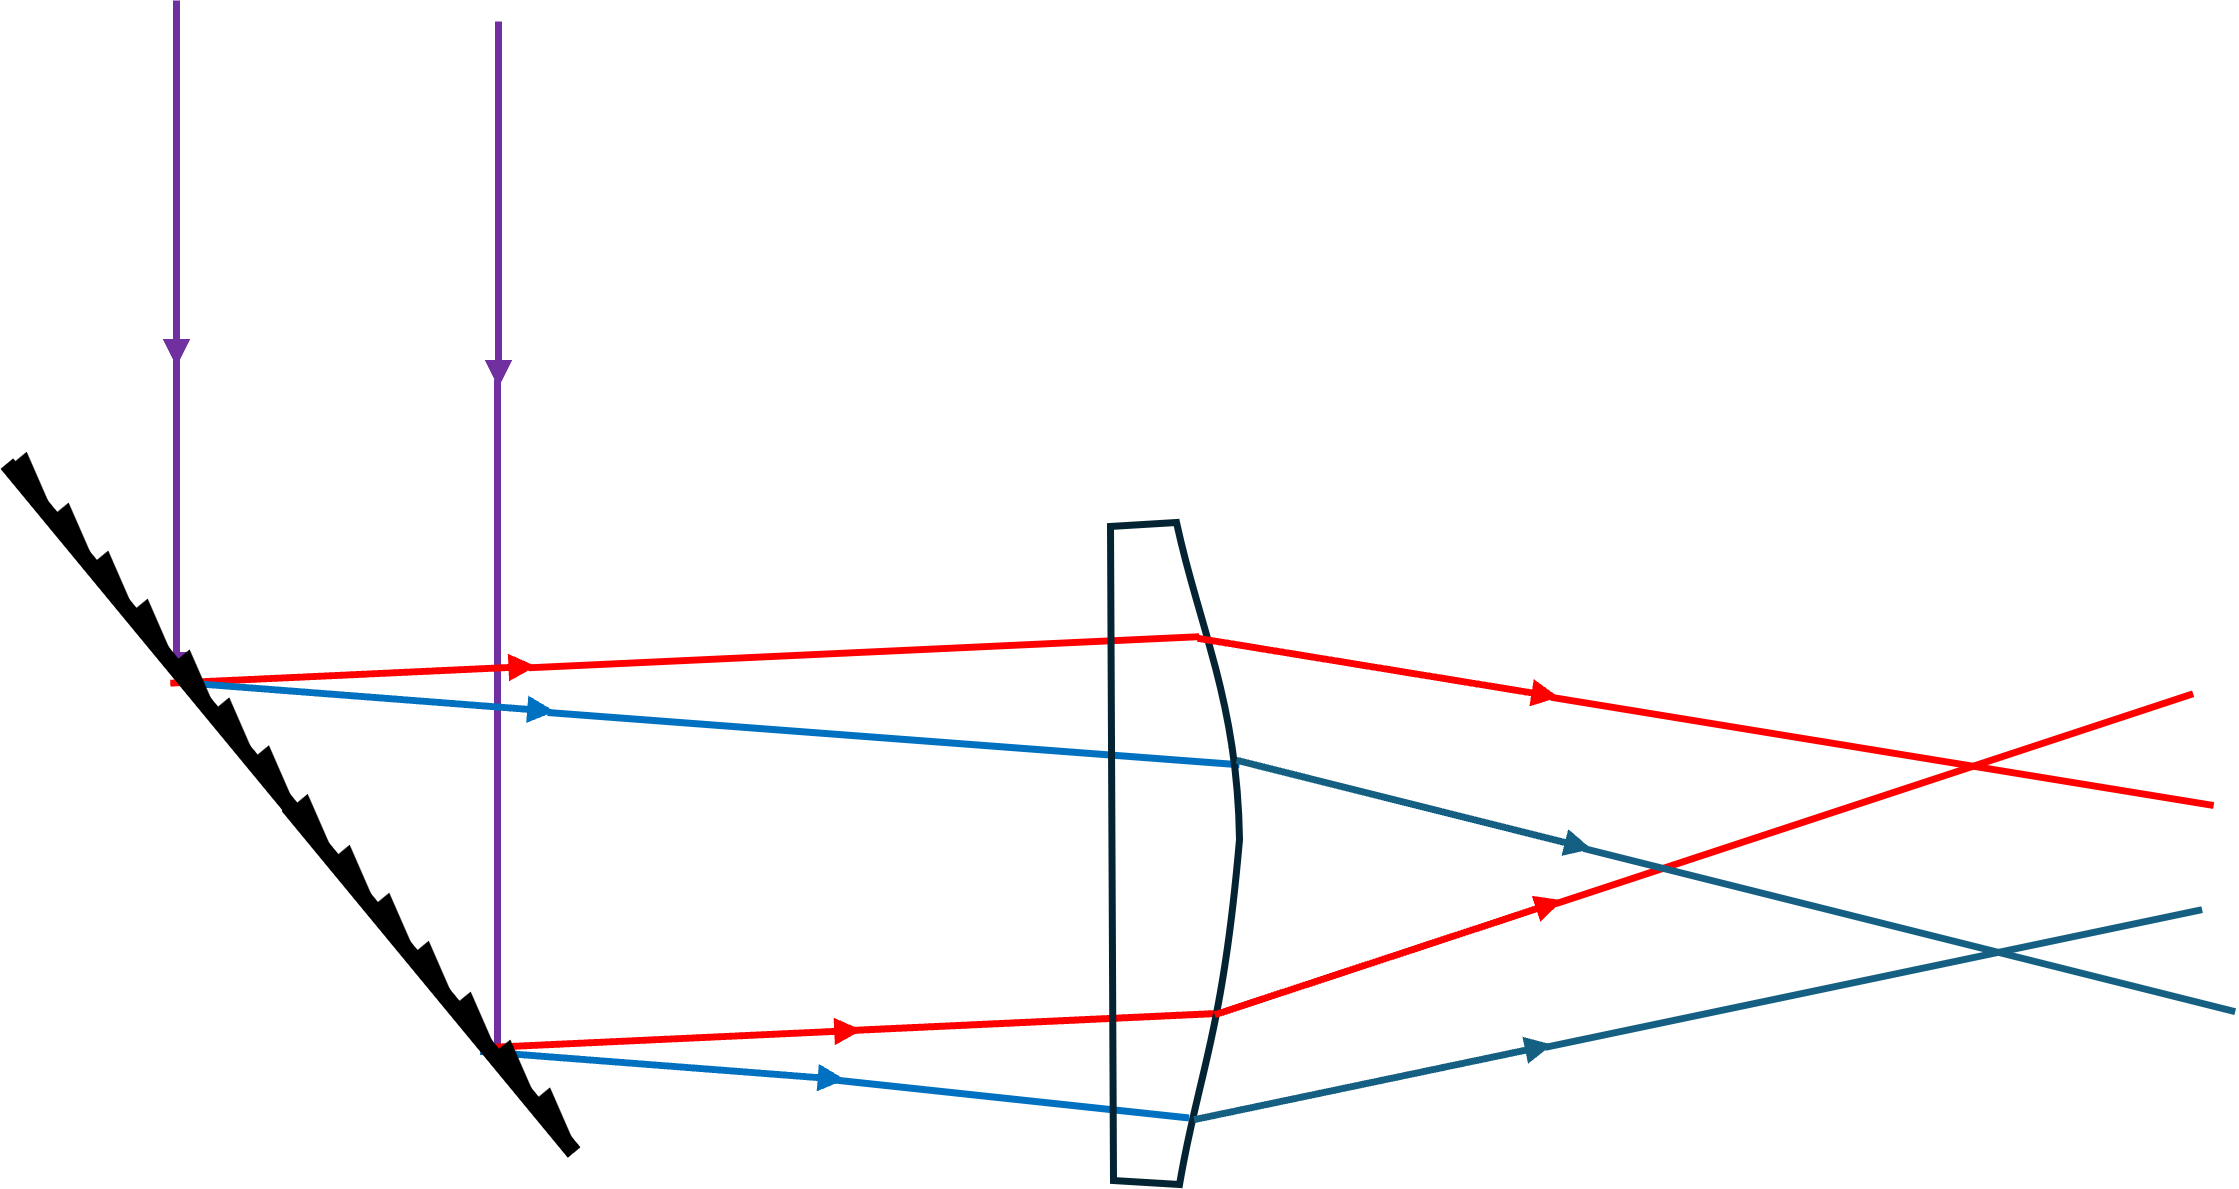
\includegraphics[width=10cm]{image/2-dispersion.png}
  \caption{波長分光の概要}
\end{figure}
\subsection{回折格子による平面波化}\label{sec:grating2}
回折格子は図(\ref{fig:doublepulse})のようにブレードと呼ばれる溝が掘られている。
光波はブレードによって反射されるが、隣り合うブレードから反射される光波は干渉を起こし、平面波となる。
このような平面波化はフーリエ変換として理解できる。
タンデム型アンジュレータから放射されるダブルパルス型の放射光が回折格子によって平面波化されることで、前後のパルスが干渉を起こす。
\subsection{電子ビームの集団運動}
これまでの議論は電子1個の場合について述べたが、実際には電子ビームは多数の電子からなり、放射光もその一つ一つから放射されるパルスの重ね合わせである。
そのため、異なる電子から放射されたパルス同士が干渉することも考慮しなければいけないが、自己相関の干渉項以外はランダム性から無視できると考えられる。
\subsection{撮影画像}
これらの一連の流れを図(??)に示した。
\begin{figure}[b]
  \centering
  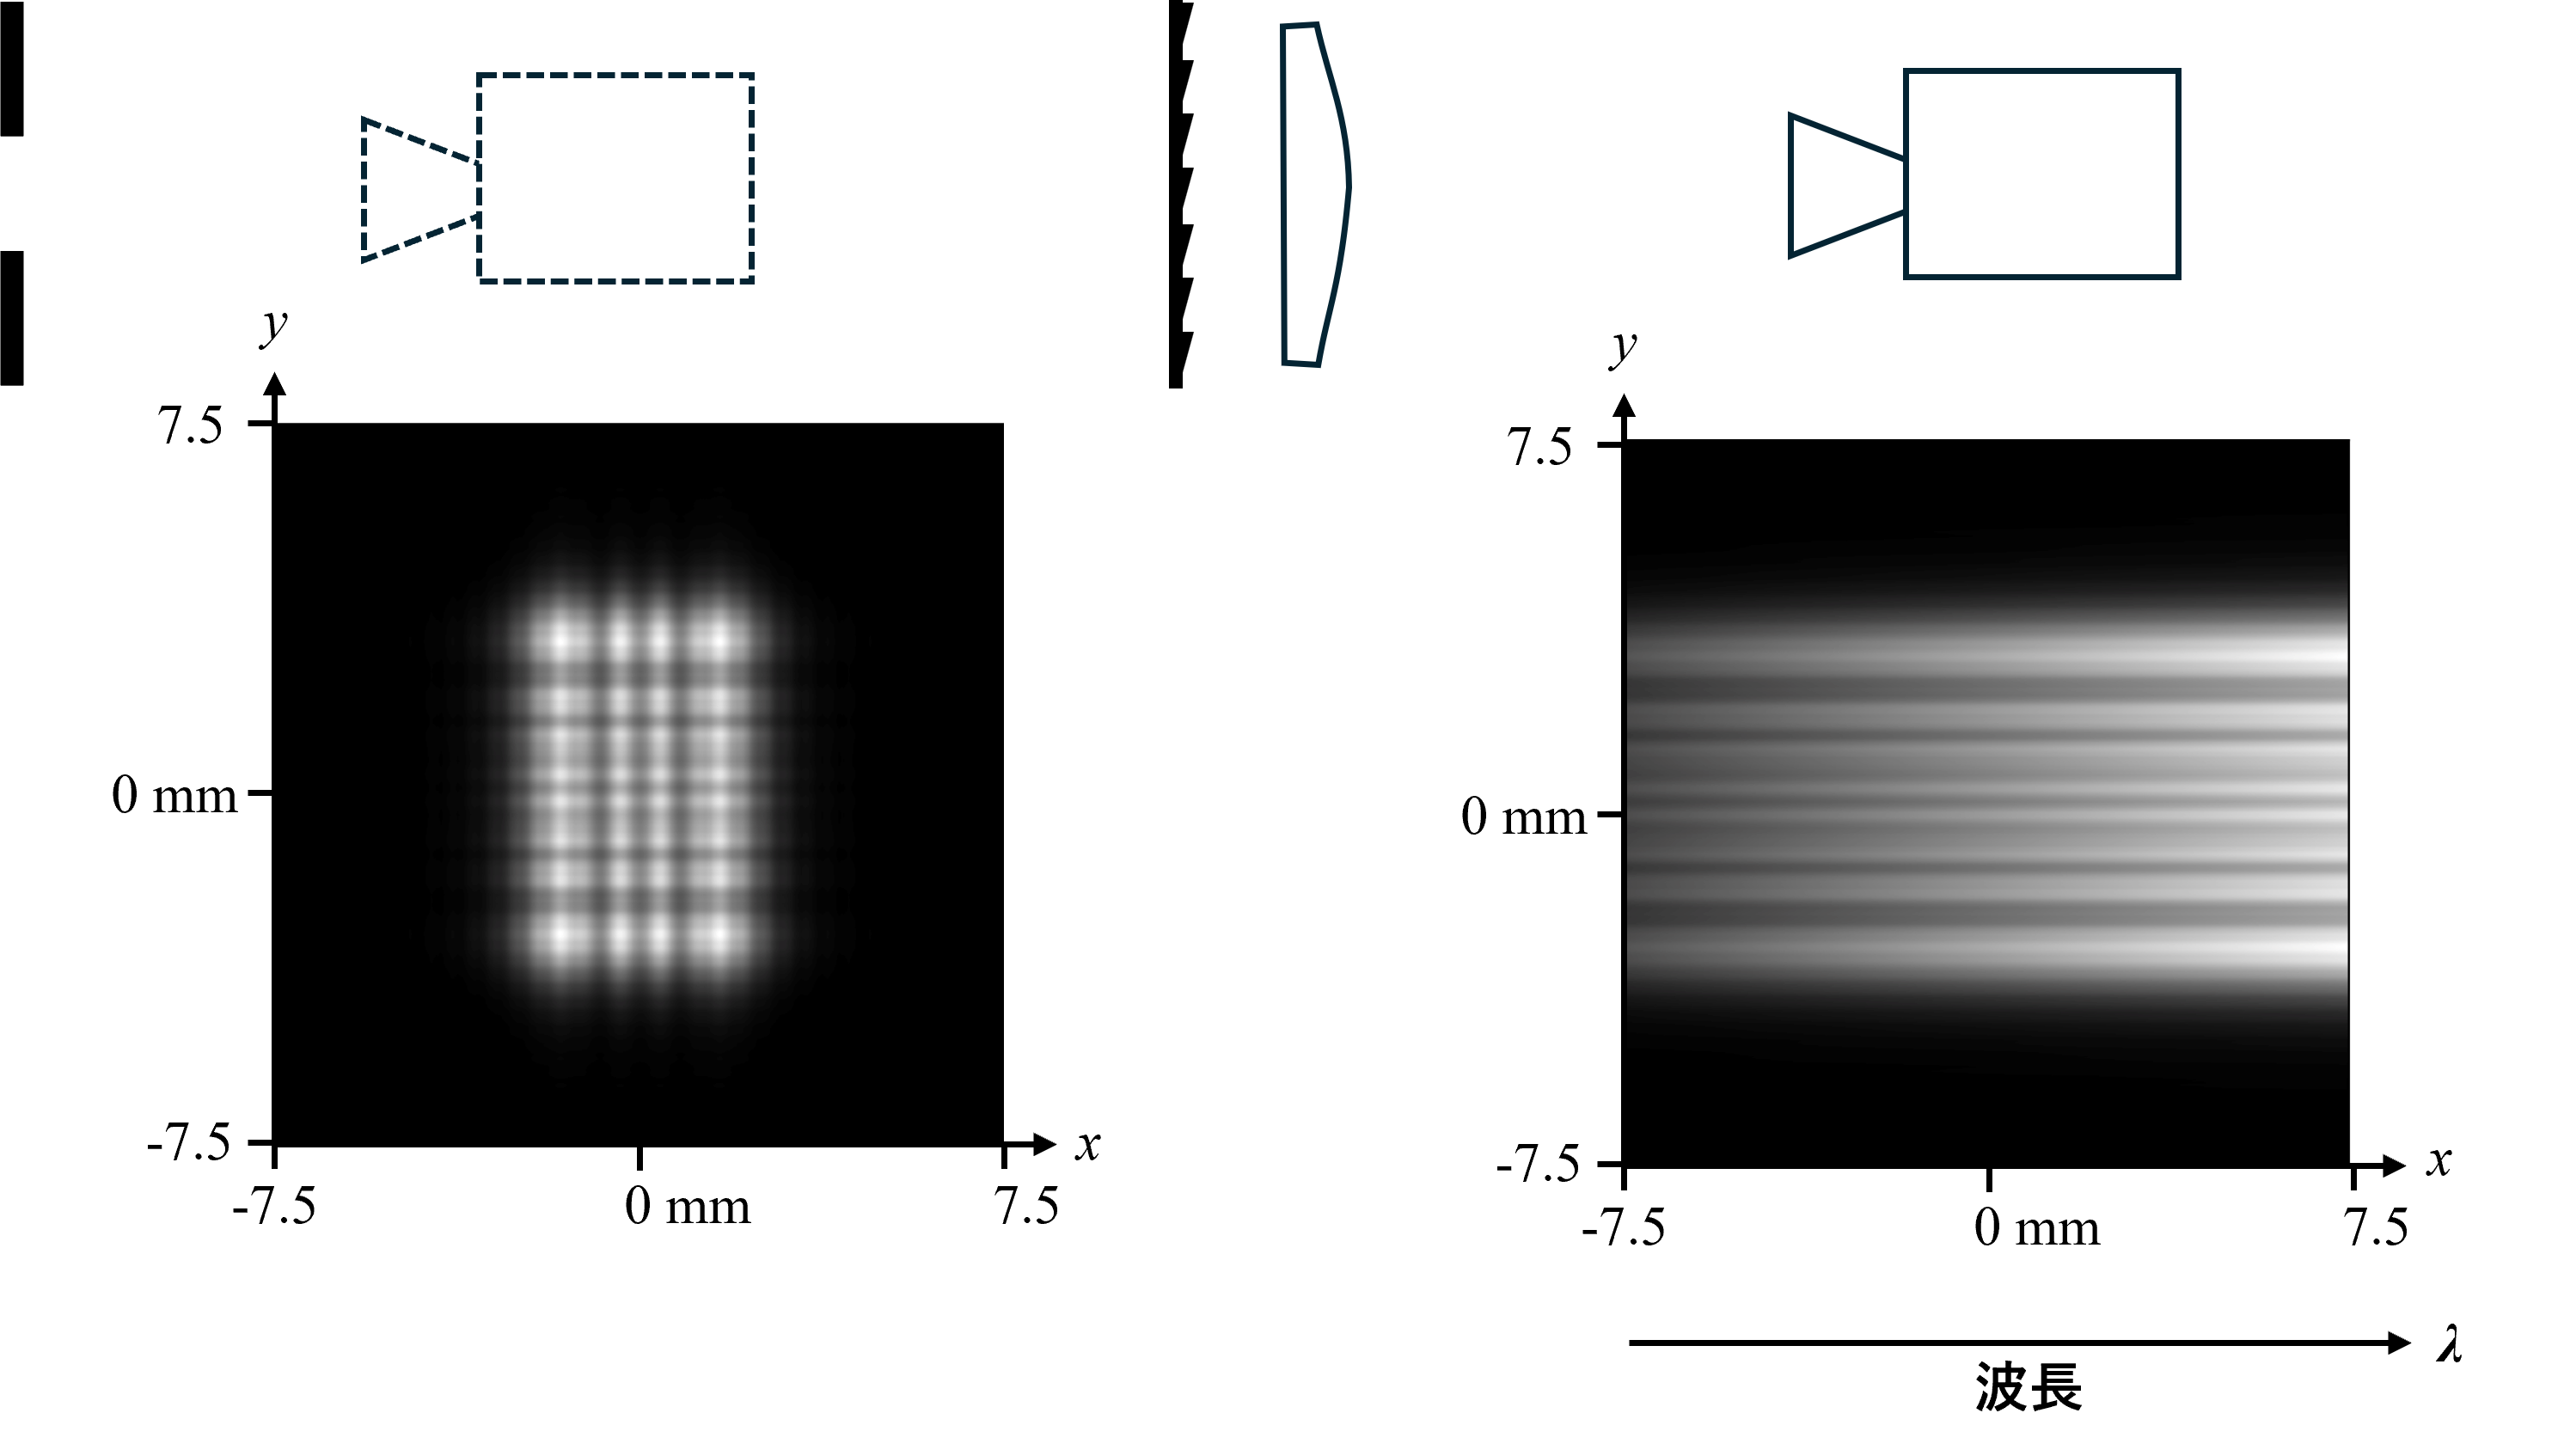
\includegraphics[width=10cm]{image/2-propagation.png}
  \caption[撮影画像の概要]{撮影画像の概要。スリットによる回折の縞模様が、回折格子で水平方向にのみ平面波化される結果、水平方向の縞模様の画像が得られる。}
\end{figure}
放射光がスリットによって回折を受けると、カメラでは2次元の回折パターン構造が得られると推定される。
一方で回折格子による分光、平面波化作用は水平方向にのみ作用する。従って画像の横軸は波長に対応し、縦軸の座標は観測角に対応する。
\subsection{モデル関数}
モデル関数の概要を示す。
モデル関数は、アンジュレータの位置座標とカメラにおけるy座標の関数として定義され、カメラの撮影画像を再現する。
放射光関数と光学関数の2つの関数に分離される。
放射光関数は、電子ビームとアンジュレータのパラメータを入力としてスリット直前の入射光の振幅および位相を計算する。
振幅は式\ref{eq:spectrum}によって計算され、位相はアンジュレータの位置を光源とした球面波位相$\exp(-ikr)$を仮定する。
光学関数は、入射光の位相と振幅を入力としてスクリーンにおける回折光の振幅を計算する。水平方向には平面波化されるため、回折積分は$y$軸方向にのみ行われる。

撮影画像を再現する最も確からしいパラメータの組を求めることで、電子ビームのエネルギーが決定できる。
\end{document}
